
\documentclass[spanish, 11pt]{exam}

%These tell TeX which packages to use.
\usepackage{array,epsfig}
\usepackage{amsmath, textcomp}
\usepackage{amsfonts}
\usepackage{amssymb}
\usepackage{amsxtra}
\usepackage{amsthm}
\usepackage{mathrsfs}
\usepackage{color}
\usepackage{multicol, xparse}
\usepackage{verbatim}


\usepackage[utf8]{inputenc}
\usepackage[spanish]{babel}
\usepackage{eurosym}

\usepackage{graphicx}
\graphicspath{{../img/}}



\printanswers
\nopointsinmargin
\pointformat{}

%Pagination stuff.
%\setlength{\topmargin}{-.3 in}
%\setlength{\oddsidemargin}{0in}
%\setlength{\evensidemargin}{0in}
%\setlength{\textheight}{9.in}
%\setlength{\textwidth}{6.5in}
%\pagestyle{empty}

\let\multicolmulticols\multicols
\let\endmulticolmulticols\endmulticols
\RenewDocumentEnvironment{multicols}{mO{}}
 {%
  \ifnum#1=1
    #2%
  \else % More than 1 column
    \multicolmulticols{#1}[#2]
  \fi
 }
 {%
  \ifnum#1=1
  \else % More than 1 column
    \endmulticolmulticols
  \fi
 }
\renewcommand{\solutiontitle}{\noindent\textbf{Sol:}\enspace}

\newcommand{\samedir}{\mathbin{\!/\mkern-5mu/\!}}

\newcommand{\class}{4º ESO}
\newcommand{\examdate}{\today}

\newcommand{\tipo}{A}


\newcommand{\timelimit}{50 minutos}



\pagestyle{head}
\firstpageheader{
\includegraphics[width=0.2\columnwidth]{header_left}}{\textbf{Departamento de Matemáticas\linebreak \class}\linebreak \examnum}{
\includegraphics[width=0.1\columnwidth]{header_right}}
\runningheader{\class}{\examnum}{Página \thepage\ of \numpages}
\runningheadrule

\newcommand{\examnum}{Autoevaluación - Trimestre 3}
\begin{document}
\begin{questions}

%\question Representa y calcula las coordenadas de las siguientes combinaciones de $\overrightarrow{u}$ y $\overrightarrow{v}$:\begin{parts} \part[1] $2 \overrightarrow{u} - 3 \overrightarrow{v}$, $- 2 \overrightarrow{u}$, $- 2 \overrightarrow{u} - 2 \overrightarrow{v}$. Siendo $\overrightarrow{u}$ y $\overrightarrow{v}$: \\ \scalebox{.65}{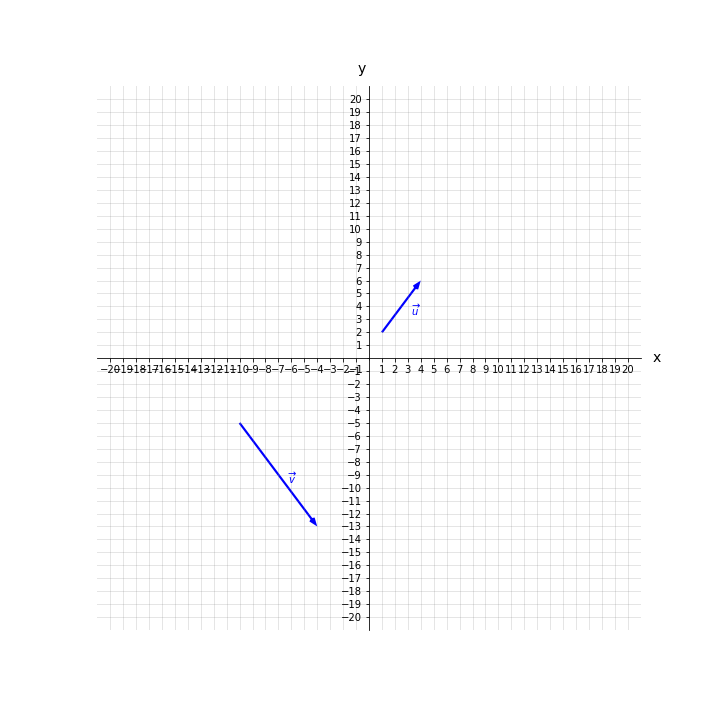
\includegraphics[width=1\columnwidth]{comb_vectores_0.png}}\begin{solution} $2 \overrightarrow{u} - 3 \overrightarrow{v}$, $- 2 \overrightarrow{u}$, $- 2 \overrightarrow{u} - 2 \overrightarrow{v}$\end{solution} \end{parts}

\question Responde a las siguientes cuestiones:\begin{parts} \part[1] Las calificaciones de un grupo de 34 alumnos han sido: 9 6 5 0 1 5 7 9 10 7 5 1 2 5 7 6 3 4 6 8 8 6 4 4 6 5 3 5 7 7 8 7 2 2. \begin{itemize} \item Realiza una tabla de frecuencias \item Realiza un diagrama de barras \item Calcular los parámetros de centralización \item Calcular los parámetros de posición P70, Q1, Q3 \item Calcular los parámetros de dispersión \item Realiza un diagrama de caja. \end{itemize}\begin{solution} $\begin{tabular}{rrrrrrr}
\hline
   $x_i$ &   $f_i$ &   $F_i$ &      \%_i &     \%A_i &   $x_if_i$ &   $x^2_if_i$ \\
\hline
       0 &       1 &       1 &   2.94118 &   2.94118 &          0 &            0 \\
       1 &       2 &       3 &   5.88235 &   8.82353 &          2 &            2 \\
       2 &       3 &       6 &   8.82353 &  17.6471  &          6 &           12 \\
       3 &       2 &       8 &   5.88235 &  23.5294  &          6 &           18 \\
       4 &       3 &      11 &   8.82353 &  32.3529  &         12 &           48 \\
       5 &       6 &      17 &  17.6471  &  50       &         30 &          150 \\
       6 &       5 &      22 &  14.7059  &  64.7059  &         30 &          180 \\
       7 &       6 &      28 &  17.6471  &  82.3529  &         42 &          294 \\
       8 &       3 &      31 &   8.82353 &  91.1765  &         24 &          192 \\
       9 &       2 &      33 &   5.88235 &  97.0588  &         18 &          162 \\
      10 &       1 &      34 &   2.94118 & 100       &         10 &          100 \\
     nan &      34 &     nan & 100       & nan       &        180 &         1158 \\
\hline
\end{tabular}$\\ 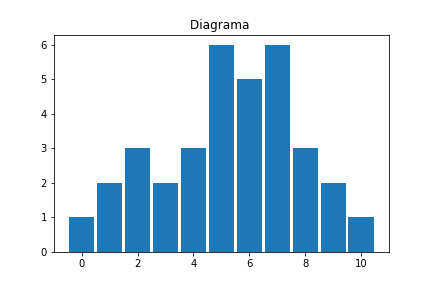
\includegraphics[width=0.7\columnwidth]{diagrama_prueba0} \\ $\left\{ Me : 5.5, \  Mo : \left( [5], \  [6]\right), \  media : 5.29\right\}$ \\$\left\{ P70 : 7.0, \  Q1 : 4.0, \  Q3 : 7.0\right\}$ \\$\left\{ C.V : 0.46, \  desv.tip : 2.46, \  rango : 10, \  var : 6.03\right\}$\\ 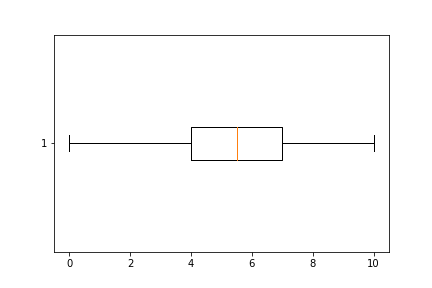
\includegraphics[width=0.7\columnwidth]{caja_prueba0}\end{solution} \part[1] Dada la siguiente distribución de datos: 0 1 1 2 2 6 6 7 7 7 2 3 3 3 4 7 8 8 8 8 4 4 5 5 5 9 9 9 10 10. \begin{itemize} \item Realiza una tabla de frecuencias \item Realiza un diagrama de barras \item Calcular los parámetros de centralización \item Calcular los parámetros de posición P70, Q1, Q3 \item Calcular los parámetros de dispersión \item Realiza un diagrama de caja. \end{itemize}\begin{solution} $\begin{tabular}{rrrrrrr}
\hline
   $x_i$ &   $f_i$ &   $F_i$ &      \%_i &     \%A_i &   $x_if_i$ &   $x^2_if_i$ \\
\hline
       0 &       1 &       1 &   3.33333 &   3.33333 &          0 &            0 \\
       1 &       2 &       3 &   6.66667 &  10       &          2 &            2 \\
       2 &       3 &       6 &  10       &  20       &          6 &           12 \\
       3 &       3 &       9 &  10       &  30       &          9 &           27 \\
       4 &       3 &      12 &  10       &  40       &         12 &           48 \\
       5 &       3 &      15 &  10       &  50       &         15 &           75 \\
       6 &       2 &      17 &   6.66667 &  56.6667  &         12 &           72 \\
       7 &       4 &      21 &  13.3333  &  70       &         28 &          196 \\
       8 &       4 &      25 &  13.3333  &  83.3333  &         32 &          256 \\
       9 &       3 &      28 &  10       &  93.3333  &         27 &          243 \\
      10 &       2 &      30 &   6.66667 & 100       &         20 &          200 \\
     nan &      30 &     nan & 100       & nan       &        163 &         1131 \\
\hline
\end{tabular}$\\ 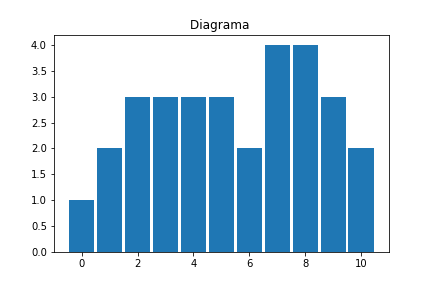
\includegraphics[width=0.7\columnwidth]{diagrama_prueba1} \\ $\left\{ Me : 5.5, \  Mo : \left( [7], \  [4]\right), \  media : 5.43\right\}$ \\$\left\{ P70 : 7.299999999999997, \  Q1 : 3.0, \  Q3 : 8.0\right\}$ \\$\left\{ C.V : 0.53, \  desv.tip : 2.86, \  rango : 10, \  var : 8.18\right\}$\\ 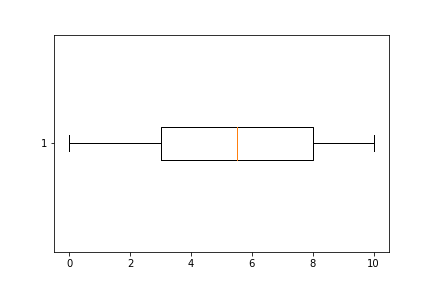
\includegraphics[width=0.7\columnwidth]{caja_prueba1}\end{solution} \part[1] Se ha preguntado a los estudiantes de una clase por el número de personas que viven en casa. Los resultados son: 3 5 4 5 8 3 5 6 4 5 4 4 3 4 5 6 5 6 4 3 4 4 5 7 4 3 4 4 6 7. \begin{itemize} \item Realiza una tabla de frecuencias \item Realiza un diagrama de barras \item Calcular los parámetros de centralización \item Calcular los parámetros de posición P70, Q1, Q3 \item Calcular los parámetros de dispersión \item Realiza un diagrama de caja. \end{itemize}\begin{solution} $\begin{tabular}{rrrrrrr}
\hline
   $x_i$ &   $f_i$ &   $F_i$ &      \%_i &    \%A_i &   $x_if_i$ &   $x^2_if_i$ \\
\hline
       3 &       5 &       5 &  16.6667  &  16.6667 &         15 &           45 \\
       4 &      11 &      16 &  36.6667  &  53.3333 &         44 &          176 \\
       5 &       7 &      23 &  23.3333  &  76.6667 &         35 &          175 \\
       6 &       4 &      27 &  13.3333  &  90      &         24 &          144 \\
       7 &       2 &      29 &   6.66667 &  96.6667 &         14 &           98 \\
       8 &       1 &      30 &   3.33333 & 100      &          8 &           64 \\
     nan &      30 &     nan & 100       & nan      &        140 &          702 \\
\hline
\end{tabular}$\\ 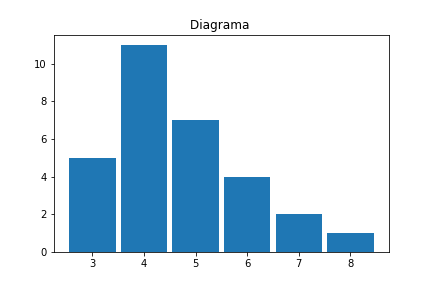
\includegraphics[width=0.7\columnwidth]{diagrama_prueba2} \\ $\left\{ Me : 4.0, \  Mo : \left( [4], \  [11]\right), \  media : 4.67\right\}$ \\$\left\{ P70 : 5.0, \  Q1 : 4.0, \  Q3 : 5.0\right\}$ \\$\left\{ C.V : 0.27, \  desv.tip : 1.27, \  rango : 5, \  var : 1.62\right\}$\\ 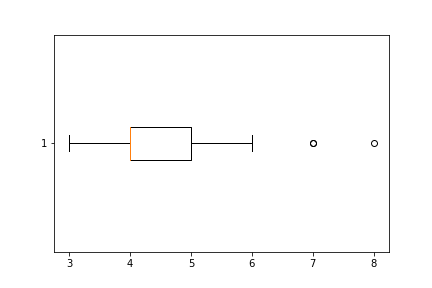
\includegraphics[width=0.7\columnwidth]{caja_prueba2}\end{solution} \end{parts} 


 
 




\end{questions}


\end{document}
